\section{Resultados e discussão}
\label{sec:resultados}
\subsection{Ajuste e resposta temporal das sinalizações}
O AE completou 200 épocas, selecionando o estado da última época, com MSE de validação interna de 0,10244. A perda interna caiu de 0,16801 na primeira época para esse valor final, acompanhando a redução da perda de treino de 0,25991 para 0,10239. O ajuste utilizou 132.718.736 transações, com 14.794.169 reservadas para validação interna. O IF foi ajustado em 500.637 transações e produziu escores, assim como o AE, para os 523.937.952 registros do ano. O treinamento do AE levou 2h13min44s e o do IF, 9,16s; a inferência anual consumiu 4min32s e 14min19s, respectivamente, em uma RTX 3060 para o AE e oito threads de CPU para o IF. Os tempos das etapas incluem as verificações de suas saídas.

Os limiares de referência Q99,5 foram $\tau_{AE}=0{,}42453$ e $\tau_{IF}=0{,}58162$. A Tabela~\ref{tab:sinalizacao} mostra que cortes congelados produzem volumes diferentes entre períodos. No teste, o AE sinalizou 4.207.945 transações (1,746\%) e o IF, 2.557.613 (1,061\%). A interseção reuniu 956.106 registros, e a união, 5.809.452, com Jaccard de 0,165. Assim, os métodos compartilham uma parcela dos registros, mas cada um acrescenta um conjunto expressivo à investigação.

\begin{table}[htbp]
\centering\small
\caption{Sinalização em Q99,5. A interseção reúne todas as transações sinalizadas pelos dois modelos, associadas ou não a bots MEV.}
\label{tab:sinalizacao}
\begin{tabular}{@{}lrrrr@{}}
\toprule
Recorte & AE (\%) & IF (\%) & Interseção & Jaccard \\
\midrule
Treino & 0,858 & 0,411 & 163.048 & 0,095 \\
Pectra & 0,872 & 0,468 & 70.072 & 0,142 \\
Validação & 0,500 & 0,500 & 40.424 & 0,107 \\
Teste & 2,583 & 1,156 & 1.024.167 & 0,128 \\
Fusaka/BPO1 & 10,539 & 1,453 & 109.941 & 0,069 \\
Estresse & 17,385 & 2,667 & 523.147 & 0,075 \\
\bottomrule
\end{tabular}
\end{table}


\begin{figure}[htbp]
\centering
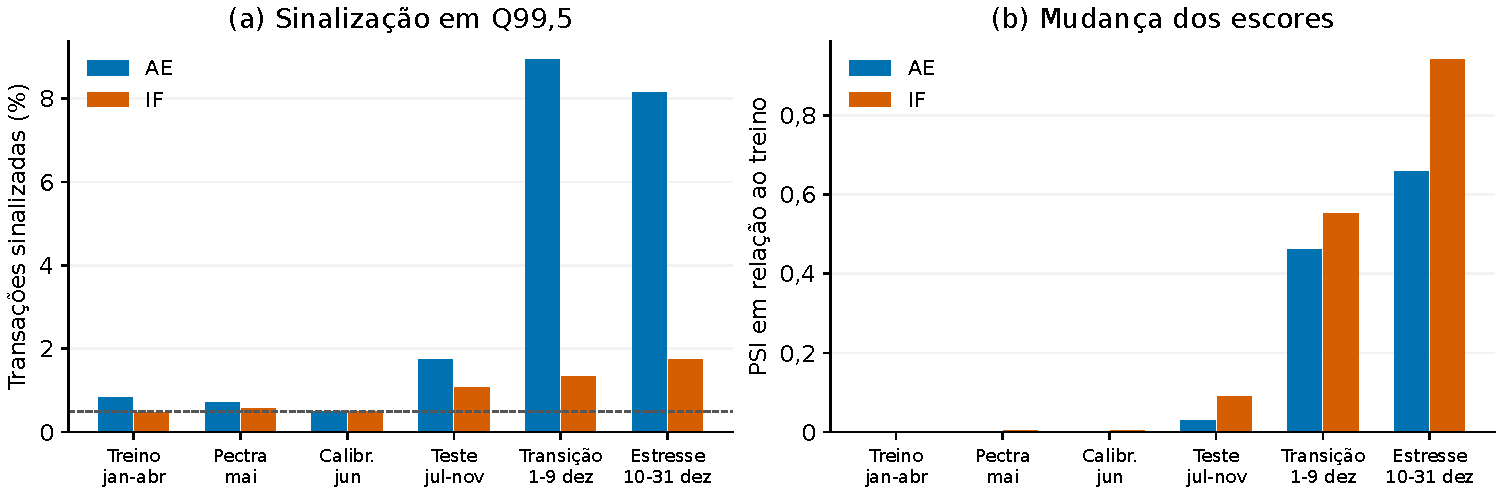
\includegraphics[width=\linewidth]{imagens/resposta-temporal.pdf}
\caption{Sinalização em Q99,5 e PSI dos escores em relação ao treino. Junho define os limiares; maio é retrospectivo. Os pontos representam recortes de durações distintas.}
\label{fig:temporal}
\end{figure}

Na transição Fusaka/BPO1, a taxa do AE alcançou 8,943\%, e a do IF, 1,335\%; no estresse, foram 8,148\% e 1,745\%. Em relação à calibração nominal de 0,5\%, o estresse expandiu a sinalização aproximadamente 16,3 vezes no AE e 3,5 vezes no IF. O comportamento também ocorre nos outros cortes: em Q99, as taxas no estresse foram 11,147\% e 2,936\%; em Q99,9, 3,018\% e 0,314\%. A expansão do AE, portanto, persiste em diferentes níveis de seletividade.

A Figura~\ref{fig:temporal} relaciona essa resposta às mudanças dos escores. Do teste ao estresse, o PSI passou de 0,030 para 0,657 no AE e de 0,090 para 0,941 no IF. Embora o IF tenha maior PSI dos escores no estresse, o AE apresenta maior expansão da taxa sinalizada. O PSI considera a distribuição nos intervalos de referência, enquanto a decisão depende da massa acima de um corte específico. A leitura conjunta evita equiparar mudança global de distribuição a crescimento da cauda sinalizada. Nos atributos, o PSI do preço efetivo passou de 0,763 no teste para 2,958 no estresse, e o da taxa máxima, de 0,452 para 1,606, contextualizando a mudança do regime transacional.

\subsection{Interseções e contribuição exclusiva dos modelos}
\begin{table}[htbp]
\centering\small
\caption{Transações associadas a bots MEV sinalizadas em Q99,5.}
\label{tab:mev-bot}
\begin{tabular}{@{}lrrrr@{}}
\toprule
Recorte & AE & IF & Interseção & União \\
\midrule
Treino & 6.249 & 8.097 & 3.074 & 11.272 \\
Pectra & 9.544 & 6.420 & 3.193 & 12.771 \\
Validação & 23.010 & 23.769 & 8.920 & 37.859 \\
Teste & 544.738 & 757.192 & 350.857 & 951.073 \\
Fusaka/BPO1 & 35.508 & 10.800 & 5.607 & 40.701 \\
Estresse & 75.354 & 13.313 & 5.014 & 83.653 \\
\bottomrule
\end{tabular}
\end{table}

A Tabela~\ref{tab:mev-bot} decompõe as transações associadas a \texttt{mev\_bot} sinalizadas em Q99,5. No teste, o AE recuperou 544.738 associadas, e o IF, 757.192. Os modelos compartilharam 350.857 associadas; 193.881 foram exclusivas do AE e 406.335, do IF. A união alcançou 951.073, correspondentes a 21,22\% das 4.481.039 transações associadas do recorte. Em comparação com o IF isolado, a união acrescentou 25,61\% de associadas recuperadas, com crescimento do conjunto investigado de 2.557.613 para 5.809.452 registros.

\begin{figure}[htbp]
\centering
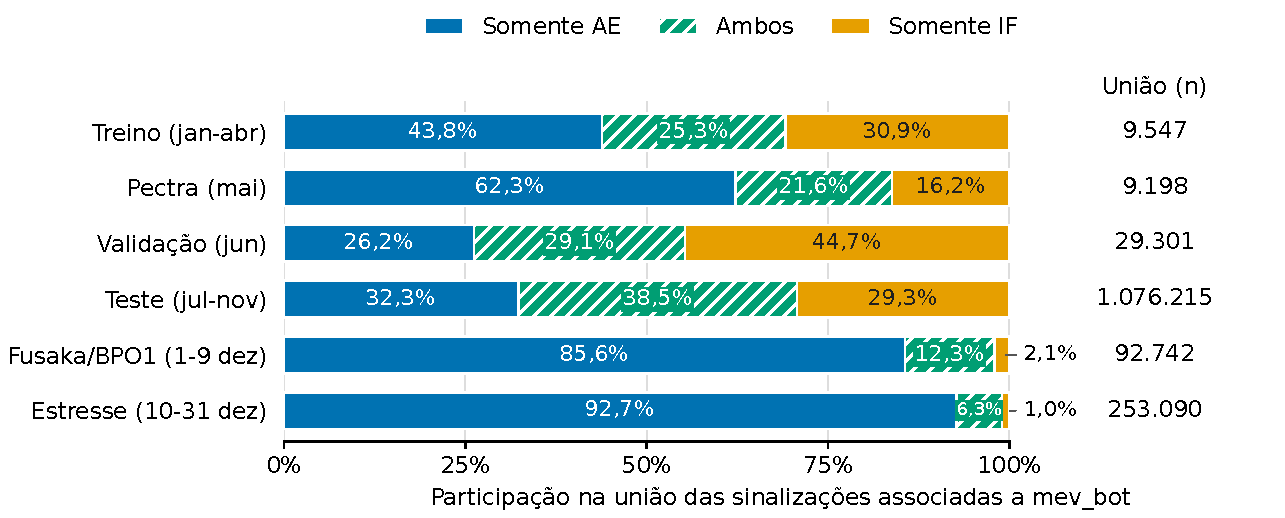
\includegraphics[width=\linewidth]{imagens/intersecoes-mev-q995.pdf}
\caption{Composição das transações associadas a \texttt{mev\_bot} sinalizadas em Q99,5. Cada barra corresponde à união associada do recorte; a coluna à direita informa sua quantidade absoluta.}
\label{fig:intersecoes}
\end{figure}

A interseção oferece outra política de priorização: as 350.857 associadas representam 36,70\% das 956.106 sinalizações compartilhadas no teste, frente a 12,95\% no conjunto do AE e 29,61\% no do IF. Sua concentração é aproximadamente 19,74 vezes a prevalência de 1,859\% no recorte. A união aumenta a recuperação, enquanto a interseção reduz o volume e eleva a concentração da referência histórica. Esses números permitem dimensionar o ganho e o custo de combinar os modelos.

A composição varia entre regimes (Figura~\ref{fig:intersecoes}). No teste, 20,4\% da união associada são exclusivos do AE, 36,9\% compartilhados e 42,7\% exclusivos do IF. No estresse, essas parcelas passam para 84,1\%, 6,0\% e 9,9\%. O AE recuperou 75.354 associadas, contra 13.313 do IF; a união alcançou 83.653, ou 25,65\% da referência do período. O IF acrescentou 8.299 associadas ao conjunto do AE, ganho de 11,01\%. Nessa janela, a interseção concentrou 2,25\% de associadas, abaixo dos 2,49\% do AE isolado: concordância entre detectores não assegura maior concentração em todos os regimes.

Na transição de dezembro, o AE recuperou 35.508 associadas e o IF, 10.800, compartilhando 5.607; a união reuniu 40.701, com recall de 28,26\%. As três janelas posteriores à calibração mostram, assim, contribuições distintas: o IF predomina entre as associadas exclusivas no teste, enquanto o AE predomina em dezembro. A combinação deve ser interpretada por período e pelo orçamento de investigação, e não como uma regra de superioridade invariável.

\subsection{Ordenação global e orçamento de investigação}
\begin{table}[htbp]
\centering\small
\caption{Ordenação dos escores frente à associação MEV. $P@1\%$ é a precision nos 1\% maiores escores; Prev. é a prevalência (\%).}
\label{tab:associacao}
\begin{tabular}{@{}lrrrrrrr@{}}
\toprule
 & & \multicolumn{2}{c}{ROC-AUC} & \multicolumn{2}{c}{AP} & \multicolumn{2}{c}{$P@1\%$ (\%)} \\ Recorte & Prev. & AE & IF & AE & IF & AE & IF \\
\midrule
Treino & 0,859 & 0,6432 & 0,9129 & 0,0128 & 0,0442 & 0,58 & 1,22 \\
Pectra & 1,028 & 0,7132 & 0,9210 & 0,0277 & 0,0633 & 4,29 & 4,12 \\
Validação & 1,273 & 0,8111 & 0,9421 & 0,1076 & 0,1219 & 19,87 & 15,79 \\
Teste & 1,859 & 0,7690 & 0,9481 & 0,0866 & 0,2067 & 8,17 & 29,26 \\
Fusaka/BPO1 & 1,010 & 0,6189 & 0,9040 & 0,0329 & 0,0524 & 8,85 & 5,67 \\
Estresse & 0,876 & 0,6309 & 0,8822 & 0,0286 & 0,0349 & 7,12 & 1,71 \\
\bottomrule
\end{tabular}
\end{table}

A Tabela~\ref{tab:associacao} reúne ROC-AUC, AP e precision nos 1\% maiores escores. O IF apresentou maior ROC-AUC e AP em todos os recortes. No teste, sua ROC-AUC foi 0,9481, contra 0,7690 do AE, e sua AP, 0,2067, contra 0,0866. Sob o mesmo orçamento de 2.410.204 transações, o IF priorizou 705.170 associadas e o AE, 196.885: precision de 29,26\% e 8,17\%, respectivamente. Os lifts foram 15,74 e 4,39 em relação à prevalência do período.

\begin{figure}[htbp]
\centering
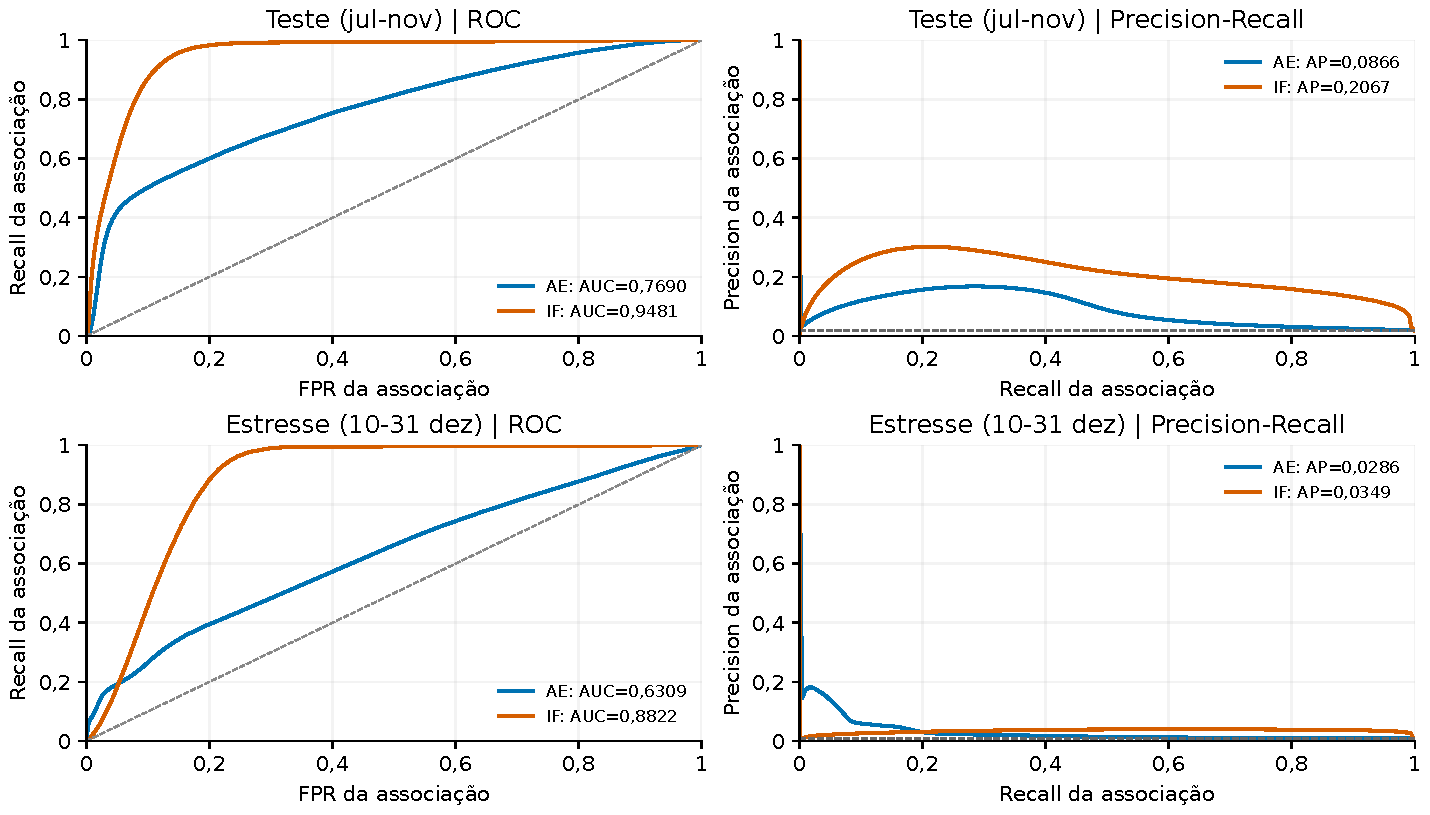
\includegraphics[width=.94\linewidth]{imagens/curvas-teste-estresse.pdf}
\caption{ROC e Precision-Recall no teste e no estresse. As linhas horizontais em Precision-Recall indicam a prevalência de cada recorte. ROC-AUC e AP são calculadas com todos os grupos de escores, antes da redução de pontos para apresentação.}
\label{fig:curvas}
\end{figure}

No estresse, a AP do IF permaneceu superior (0,0349 frente a 0,0286), assim como a ROC-AUC (0,8822 frente a 0,6309). Entretanto, nos 1\% maiores escores, o AE concentrou 7,12\% de associadas, e o IF, 1,71\%, para prevalência de 0,876\%. O AE priorizou 26.492 associadas nesse orçamento, contra 6.371 do IF. A Figura~\ref{fig:curvas} evidencia que as curvas Precision-Recall podem favorecer métodos diferentes em regiões distintas de recall. A AP resume a ordenação em seu conjunto; a precision sob orçamento fixo descreve uma decisão operacional específica.

\begin{figure}[htbp]
\centering
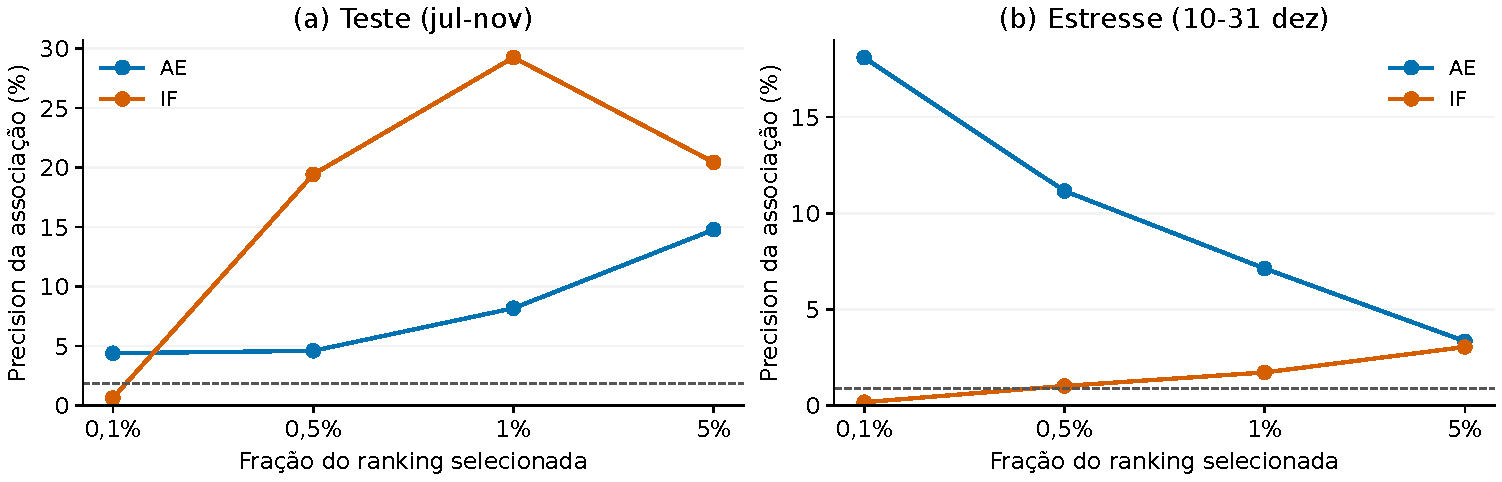
\includegraphics[width=\linewidth]{imagens/orcamento-investigacao.pdf}
\caption{Precision da associação MEV em quatro orçamentos fixos do ranking. Linhas tracejadas indicam a prevalência. O mesmo percentual seleciona a mesma quantidade de transações para ambos os modelos em cada recorte.}
\label{fig:orcamento}
\end{figure}

A Figura~\ref{fig:orcamento} amplia essa comparação. No teste, o IF superou o AE nos quatro orçamentos, de 0,1\% a 5\%. No estresse, o AE apresentou maior concentração nos quatro: nos 0,1\% maiores escores, sua precision foi 18,10\%, contra 0,16\% do IF; nos 5\%, foram 3,33\% e 3,04\%. A diferença reduz-se com a ampliação do conjunto investigado. A precision não cresce necessariamente quando o corte se torna mais extremo: no teste, o AE concentra 4,38\% no topo de 0,1\%, mas 14,77\% no topo de 5\%. Logo, escores mais extremos de anormalidade não precisam coincidir com maior concentração dessa categoria histórica.

Em conjunto, os resultados respondem às três questões do estudo: limiares fixos produzem expansão temporal distinta das sinalizações; a sobreposição é parcial e sua composição muda entre recortes; e a qualidade global da ordenação não determina, sozinha, o método mais adequado a um orçamento restrito. A análise de AP, precision, recall e parcelas exclusivas permite escolher entre concentração, recuperação e volume de investigação com critérios quantitativos comuns.
